\label{chapter_kedmd}
Until now, we supposed that the number of snapshots was large compared to the size of the dictionary, which also controls the number of eigenpairs approximated. However, when dealing with high dimensional data, we are usually in the opposite regime, where $K \gg M$. Indeed, as the dimension of the state space increases, the number of functions needed to have a rich enough dictionary overgrows. This blowup of the size $K$ of the dictionary occurs frequently in data-driven and Machine Learning related applications \cite{budisic_applied_2012, rowley_spectral_2009, schmid_dynamic_2010}, and it can be regarded as a facet of the so-called \emph{curse of dimensionality} \cite{bishop_pattern_2006}.  In this final chapter, we present Kernelized EDMD (K-EDMD), an algorithm that uses the kernel trick for a more efficient computation of the EDMD approximations. Unfortunately, having a dictionary size larger than the number of quadrature points makes ResDMD non applicable. This can be solved by using the two-steps procedure presented in \Cref{section_kresdmd}. Finally, we apply the previously mentioned two-steps procedure to the Gauss iterated map problem in order to obtain approximations of the Koopman eigenvalues without the need of a hand-crafted dictionary.

\section{Kernelized EDMD (K-EDMD)}
The EDMD algorithm necessitates the computation of the matrices $(\Psi_0^*\vb*{W}\Psi_0)$ and $(\Psi_0^*\vb*{W}\Psi_1)$, which requires $\mathcal{O}(MK^2)$ flops, and solving an eigenvalue problem associated to the matrix $\vb*{K}\in\C^{K\times K}$, which costs $\mathcal{O}(K^3)$ flops. For large values of $K$, such computations are impractical. \emph{Kernelized EDMD} (K-EDMD) \cite{williams_kernel-based_2015} uses the kernel trick \cite{bishop_pattern_2006} to efficiently compute a matrix $\hat{\vb*{K}}\in\C^{M\times M}$ that has the same non-zero eigenvalues as $\vb*{K}$. The computation of such a matrix relies on the following proposition.

\begin{prop}[\cite{colbrook_rigorous_2021}]
\label{prop_kedmd}
Let $\sqrt{\vb*{W}}\Psi_0 = \vb*{Q}\vb*{\Sigma}\vb*{Z}^*$ be a SVD, where $\vb*{\Sigma}\in\C^{M\times M}$ and let us define
\begin{equation}
    \label{kedmd_matrix}
    \hat{\vb*{K}} = (\vb*{\Sigma}^{\dagger}\vb*{Q}^*)(\sqrt{\vb*{W}}\Psi_1\Psi_0\sqrt{\vb*{W}})(\vb*{Q}\Sigma^{\dagger})\in\C^{M \times M}.
\end{equation}
Then $(\lambda,\,\vb{v})$ with $\lambda\neq 0$ is an eigenpair of $\hat{\vb*{K}}$ if and only if $(\lambda,\,\vb*{Z}\vb{v})$ is an eigenpair of $\vb*{K}$, where $\vb*{K}$ is defined in \eqref{discretized_problem_solution}.
\end{prop}
\begin{proof}
Let us recall that the matrix $\vb*{K}$ is defined in \eqref{discretized_problem_solution} as $\vb*{K} = (\Psi_0^*\vb*{W}\Psi_0)^{\dagger}(\Psi_0^*\vb*{W}\Psi_1)$. For a generic matrix $\vb*{A}$, the following two properties of the Moore-Penrose inverse hold: $(\vb*{A}^*\vb*{A})^{\dagger}\vb*{A}^* = \vb*{A}^{\dagger}$ and $\range(\vb*{A}^{\dagger}) = \range(\vb*{A}^*)$, where $\range(\vb*{A})$ denotes the Span of the columns (or range) of $\vb*{A}$. Applying these two properties to the matrix $\vb*{A} = \sqrt{\vb*{W}}\Psi_0$ it follows: 
\begin{equation*}
    \begin{split}
        &\vb*{K} = (\Psi_0^*\vb*{W}\Psi_0)^{\dagger}(\Psi_0^*\vb*{W}\Psi_1) = (\sqrt{\vb*{W}}\Psi_0)^{\dagger} \sqrt{\vb*{W}}\Psi_1 \\
        &\range(\vb*{K}) \subseteq \range((\sqrt{\vb*{W}}\Psi_0)^{\dagger}) = \range(\sqrt{\vb*{W}}\Psi_0)^*)
    \end{split}
\end{equation*}
Hence any eigenvector $\vb{v}$ such that $\vb*{K}\vb{v} = \lambda \vb{v}$ with $\lambda \neq 0$ can be written as $\vb{v} = (\sqrt{\vb*{W}}\Psi_0)^*\tilde{\vb{v}} = \vb*{Z}\vb*{\Sigma}\vb*{Q}^*\tilde{\vb{v}} = \vb*{Z}\hat{\vb{v}}$ for some $\hat{\vb{v}}$. Thus:
\begin{equation*}
    \lambda \vb*{Z}\hat{\vb{v}} = \vb*{K}\vb*{Z}\hat{\vb{v}} = (\sqrt{\vb*{W}}\Psi_0)^{\dagger} \sqrt{\vb*{W}}\Psi_1 \vb*{Z}\hat{\vb{v}} = \vb*{Z}\left[(\vb*{\Sigma}^{\dagger}\vb*{Q}^*)(\sqrt{\vb*{W}}\Psi_1\Psi_0\sqrt{\vb*{W}})(\vb*{Q}\Sigma^{\dagger})\right] \hat{\vb{v}}
\end{equation*}
and multiplying by $\vb*{Z}^*$ on the right we obtain that if $(\lambda,\,\vb{v})$ is an eigenpair of $\vb*{K}$ with $\lambda\neq 0$, then $(\lambda,\,\hat{\vb{v}} = \vb*{Z}^*\vb{v})$ is an eigenpair of $\hat{\vb*{K}}$. 

Vice versa, if $(\lambda,\,\vb{v})$ is an eigenpair of $\hat{\vb*{K}}$, then:
\begin{equation*}
    \vb*{K}\vb*{Z}\vb{v} = \vb*{Z}\hat{\vb*{K}}\vb{v} = \lambda\vb*{Z}\vb{v}
\end{equation*}
i.e. $(\lambda,\,\vb*{Z}\vb{v})$ is an eigenpair of $\vb*{K}$.
\end{proof}

Now observe that to build the matrix $\hat{\vb*{K}}$ we just need to compute inner products of evaluation of our dictionary. The matrices $\vb*{Q}$ and $\vb*{\Sigma}$ can be obtained from the eigenvalue decomposition of $\sqrt{\vb*{W}}\Psi_0\Psi_0^*\sqrt{\vb*{W}} = \vb*{Q}\vb*{\Sigma}^2\vb*{Q}^*$, and both $(\sqrt{\vb*{W}}\Psi_0\Psi_0^*\sqrt{\vb*{W}})$ and $(\sqrt{\vb*{W}}\Psi_1\Psi_0^*\sqrt{\vb*{W}})$ can be computed using inner products only. Indeed, recalling that $\Psi(\vb{x})$ is a row vector:
\begin{equation}
    \label{kernel_matrices}
    \begin{split}
        (\sqrt{\vb*{W}}\Psi_0\Psi_0^*\sqrt{\vb*{W}})_{ij} &= \sqrt{w_i} \Psi(\vb{x}_0^{(i)}) \Psi(\vb{x}_0^{(j)})^* \sqrt{w_j}\\
        (\sqrt{\vb*{W}}\Psi_1\Psi_0^*\sqrt{\vb*{W}})_{ij} &= \sqrt{w_i} \Psi(\vb{x}_1^{(i)}) \Psi(\vb{x}_0^{(j)})^* \sqrt{w_j}.
    \end{split}
\end{equation}
The kernel trick \cite{bishop_pattern_2006} is a common technique used to compute these inner products implicitly. Instead of first evaluating the dictionary $\Psi(\vb{x})$ and then computing the inner product, that would require $\mathcal{O}(K)$ operations, we compute $\kappa(\vb{x}, \vb{y}) = \Psi(\vb{x})\Psi(\vb{y})^*$ for a suitably defined kernel $\kappa$. It is crucial that the kernel $\kappa$ does not compute the inner product directly, but it does so implicitly in $\mathcal{O}(d)$ operations, where $d$ is the data dimension. Thus the matrices $(\sqrt{\vb*{W}}\Psi_0\Psi_0^*\sqrt{\vb*{W}})$ and $(\sqrt{\vb*{W}}\Psi_1\Psi_0^*\sqrt{\vb*{W}})$ can be calculated in $\mathcal{O}(dM^2)$ operations, without suffering from the large size of the dictionary. The total complexity of computing $\hat{\vb*{K}}$ and solving the associated eigenvalue problem is $\mathcal{O}(d M^2 + M^3)$, significantly lower than the $\mathcal{O}(M K^2+K^3)$ cost of applying EDMD directly. 

\subsection{Computing the Koopman eigenvalues, eigenfunctions and modes}
Once we have computed the matrix $\hat{\vb*{K}}$ and its eigendecomposition, we still need to understand how to retrieve from it an approximation of the Koopman eigenvalues, eigenfunctions and modes. The eigenvalues of $\hat{\vb*{K}}$ can be directly used as approximation of the Koopman eigenvalues. Let $\hat{\bm{\Xi}} = \left[\hat{\bm{\xi}}_1,\dots,\hat{\bm{\xi}}_M\right]$ be the matrix of the eigenvectors of $\hat{\vb*{K}}$, the vector of approximate Koopman eigenfunctions $\Phi(\vb{x}) = \left[\phi_1(\vb{x}), \dots, \phi_M(\vb{x})\right]$ can be written as $\Phi = \Psi\vb*{Z}\hat{\bm{\Xi}} = \Psi (\Psi_0^*\sqrt{\vb*{W}})(\vb*{Q}\Sigma^{\dagger}) \hat{\bm{\Xi}}$. All we have done so far would not be useful if we suffered from the size of the dictionary when approximating the Koopman eigenfunctions. Fortunately, it is possible to express them using kernels only. Indeed:
\begin{equation}
    \label{kernel_eigenfunctions}
    \begin{split}
        \phi_k(\vb{x}) &= \Psi(\vb{x}) (\Psi_0^*\sqrt{\vb*{W}})(\vb*{Q}\Sigma^{\dagger}) \hat{\bm{\xi}}_k =\\
        &= \left[\sqrt{w_1} \kappa(\vb{x}, \vb{x}_0^{(1)}), \dots, \sqrt{w_M} \kappa(\vb{x}, \vb{x}_0^{(M)})\right](\vb*{Q}\Sigma^{\dagger}) \hat{\bm{\xi}}_k
    \end{split}
\end{equation}
so that the size $K$ of the dictionary does not enter any of the computations.

To compute the Koopman modes of the full state observable, we consider equation \eqref{koopman_modes} and we evaluate it at each of the data points using the approximate eigenfunctions we just obtained. When evaluated at $\vb{x}_0^{(i)}$ the equation reads:
\begin{equation}
    \label{kedmd_modes_pointwise}
    \vb{x}_0^{(i)} = \sum_{j = 1}^M \phi_j(\vb{x}_0^{(i)})\hat{\vb{v}}_{j} + \vb{r}_i
\end{equation}
where $\{\hat{\vb{v}}_{j}\}_{j=1}^M$ are the Koopman modes that we want to retrieve and $\vb{r}_i$ is a residual that must be minimized. If we introduce the matrices
\begin{equation}
    \begin{split}
    \vb*{X} = 
    \begin{bmatrix}
    (\vb{x}_0^{(1)})^T \\
    \vdots \\
    (\vb{x}_0^{(M)})^T
    \end{bmatrix}&,
    \\ 
    \Phi_0 = 
    \begin{bmatrix}
    \Phi(\vb{x}_0^{(1)}) \\
    \vdots \\
    \Phi(\vb{x}_0^{(M)})
    \end{bmatrix}&
    = \Psi_0 \vb*{Z}\hat{\bm{\Xi}} = \Psi_0 (\Psi_0^*\sqrt{\vb*{W}})(\vb*{Q}\Sigma^{\dagger}) \hat{\bm{\Xi}} =\\
    & = \sqrt{\vb*{W}^{-1}} \vb*{Q}\vb*{\Sigma}^2\vb*{Q}^*\vb*{Q}\Sigma^{\dagger}\hat{\bm{\Xi}} = \sqrt{\vb*{W}^{-1}} \vb*{Q}\Sigma\hat{\bm{\Xi}}
    \end{split}
\end{equation}
i.e. the data-points matrix and the matrix of the eigenfunctions values at those points, \eqref{kedmd_modes_pointwise} can be rewritten as
\begin{equation}
    \label{kedmd_modes_matrix}
    \vb*{X} = \Psi_0 \hat{\vb*{V}} + \vb*{R}.
\end{equation}
The solution to the least squares problem is 
\begin{equation}
    \hat{\vb*{V}} =  
    \begin{bmatrix}
    \hat{\vb{v}}_1^T \\
    \vdots \\
    \hat{\vb{v}}_M^T
    \end{bmatrix}
    = \Psi_0^{\dagger} \vb*{X} = \hat{\bm{\Xi}}^{-1} \Sigma^{\dagger} \vb*{Q}^* \sqrt{\vb*{W}} \vb*{X}.
\end{equation}
Hence the approximation of the $j$-th Koopman mode is 
\begin{equation}
    \label{kedmd_modes}
    \hat{\vb{v}}_j = (\hat{\vb{u}}_j^* \Sigma^{\dagger} \vb*{Q}^* \sqrt{\vb*{W}} \vb*{X})^T
\end{equation}
where $\hat{\vb{u}}_j$ is a left eigenvector of $\hat{\vb*{K}}$ appropriately scaled so that $\hat{\vb{u}}_j^*\hat{\bm{\xi}}_i = \delta_{ij}$.

\subsection{The choice of the kernel}
Even if in the previous discussion we supposed that, given a dictionary $\Psi(\vb{x})$, there exists a kernel $\kappa$ that computes $\kappa(\vb{x}, \vb{y}) = \Psi(\vb{x})\Psi(\vb{y})^*$ implicitly, in effect it is usually the choice of $\kappa$ that defines the dictionary. One of the most simple kernels is the polynomial kernel $\kappa(\vb{x}, \vb{y}) = (1 + \vb{x}^*\vb{y})^{n}$, which is equivalent to a dictionary that can represent all polynomials up to degree $n$. Increasing $n$ the implicitly defined dictionary becomes larger, at the cost of a worst conditioning of the resulting matrices. For this reason, taking inspiration from Machine Learning techniques, other kernels could be considered, such as the widely used radial basis function kernel (RBF kernel), $\kappa(\vb{x}, \vb{y}) = \exp(-\norm{\vb{x}-\vb{y}}^2 / \sigma^2)$.

\begin{algorithm}[h]
\caption{\textbf{: Kernelized EDMD (K-EDMD)}}
\label{alg_kedmd}
\textbf{Input:} Snapshot pairs of the system state, $\{(\vb{x}_0^{(m)}, \vb{x}_1^{(m)})\}_{m = 1}^M$, quadrature weights $\{w_m\}_{m = 1}^M$, kernel $\kappa = \kappa(\cdot\,,\,\cdot)$.
\begin{algorithmic}[1]
\State  Compute the matrices $\hat{\vb*{G}} = \sqrt{\vb*{W}}\Psi_0\Psi_0^*\sqrt{\vb*{W}}$ and  $\hat{\vb*{A}} = \sqrt{\vb*{W}}\Psi_1\Psi_0^*\sqrt{\vb*{W}}$, exploiting that $\hat{\vb*{G}}_{ij} = \sqrt{w_i} \kappa(\vb{x}_0^{(i)},\, \vb{x}_0^{(j)}) \sqrt{w_j}$ and
$\hat{\vb*{A}}_{ij} = \sqrt{w_i} \kappa(\vb{x}_1^{(i)},\, \vb{x}_0^{(j)}) \sqrt{w_j}$.
\State Compute the eigenvalue decomposition of $\hat{\vb*{G}} = \vb*{Q}\vb*{\Sigma}^2\vb*{Q}^*$.
\State Compute $\hat{\vb*{K}} = (\vb*{\Sigma}^{\dagger}\vb*{Q}^*)\hat{\vb*{A}} (\vb*{Q}\Sigma^{\dagger})$.
\State Solve the eigenvalue problem of $\hat{\vb*{K}}\hat{\bm{\xi}} = \lambda \hat{\bm{\xi}}$.
\State Obtain the eigenfunctions as $\phi_k(\vb{x}) = \left[\sqrt{w_1} \kappa(\vb{x}, \vb{x}_0^{(1)}), \dots, \sqrt{w_M} \kappa(\vb{x}, \vb{x}_0^{(M)})\right](\vb*{Q}\Sigma^{\dagger}) \hat{\bm{\xi}}_k$.
\If{want to compute eigenmodes}
    \State Compute the left eigenvectors $\vb{u}_j$ of $\hat{\vb*{K}}$ appropriately scaled so that $\hat{\vb{u}}_j^*\hat{\bm{\xi}}_i = \delta_{ij}$.
    \State Compute $\hat{\vb*{B}} = \Sigma^{\dagger} \vb*{Q}^* \sqrt{\vb*{W}} \vb*{X}$.
    \State Obtain the modes as $\hat{\vb{v}}_j = (\hat{\vb{u}}_j^* \hat{\vb*{B}})^T$.
\EndIf
\end{algorithmic}
\textbf{Output:} Approximation of the eigenvalues ($\lambda_j$), eigenfunctions ($\phi_j$) and, possibly, eigemodes ($\vb{v}_j$).
\end{algorithm}

\section{Kernelized ResDMD (K-ResDMD)}
\label{section_kresdmd}
At this point, it is a natural question how one could extend ResDMD with a kernelized approach. Unfortunately, applying \Cref{alg_resdmd} with K-EDMD instead of EDMD makes the approximate residual always vanish (see \cite{colbrook_rigorous_2021}, Proposition 6.2). Basically, since the size of our function space is larger than the number of snapshots, we can "interpolate", and we are actually overfitting our dataset. Similarly to what is done when training and testing a Machine Learning model, to have a reliable estimate of the residual for approximate eigenpairs, we need to compute it using quadrature points that have not been used at the "interpolation stage" and that, at least ideally, are independent of the ones previously employed. This idea leads to the following multi-step approach:
\begin{enumerate}
    \item Split the snapshot data into two (ideally independent) sets $\{(\vb{x}_0^{(j)},\,\vb{x}_1^{(j)})\}_{j=1}^{M'}$ and  $\{(\vb{y}_0^{(j)},\,\vb{y}_1^{(j)})\}_{j=1}^{M''}$, with $M'' \geq M'$.
    \item Apply K-EDMD to the first data set $\{(\vb{x}_0^{(j)},\,\vb{x}_1^{(j)})\}_{j=1}^{M'}$, and compute a dictionary that Spans the function space generate by the approximations of dominant $K' < M'$ eigenfunctions (see \Cref{alg_kresdmd} for the details). Let us denote this dictionary as $\Psi(x) = \left[\psi_1(\vb{x}), \dots, \psi_{K'}(\vb{x})\right]$.
    \item Apply \Cref{alg_resdmd} or \Cref{alg_pseudospectrum} with snapshot data $\{(\vb{y}_0^{(j)},\,\vb{y}_1^{(j)})\}_{j=1}^{M''}$ and dictionary $\Psi(x)$.
\end{enumerate}
As summarized in \Cref{alg_kresdmd} in the first stage, we reduce the size of the dictionary implicitly defined by the kernel to $K'$, hoping to obtain a good dictionary that already captures the essential dynamics. Then this dictionary is used as a basis for the ResDMD algorithm, which computes reliable approximations of the eigenpairs of the Koopman operator. This also provides an a posteriori check of the quality of the dictionary obtained in the first stage.

\begin{algorithm}[h]
\caption{\textbf{: Kernelized ResDMD (K-ResDMD)}}
\label{alg_kresdmd}
\textbf{Input:} Snapshot pairs of the system state, $\{(\vb{x}_0^{(m)}, \vb{x}_1^{(m)})\}_{m = 1}^M$, quadrature weights $\{w_m\}_{m = 1}^M$, kernel $\kappa = \kappa(\cdot\,,\,\cdot)$, hyperparameters $M', \,M'', \,K'$.
\begin{algorithmic}[1]
\State  Split the snapshot data into $\{(\vb{x}_0^{(j)},\,\vb{x}_1^{(j)})\}_{j=1}^{M'}$ and  $\{(\vb{y}_0^{(j)},\,\vb{y}_1^{(j)})\}_{j=1}^{M''}$, with $M = M' + M''$ and $M'' \geq M' > K'$.
\State Apply K-EDMD (\Cref{alg_kedmd}) with snapshot pairs $\{(\vb{x}_0^{(j)},\,\vb{x}_1^{(j)})\}_{j=1}^{M'}$: compute the dominant $K' < M'$ eigenvectors of $\hat{\vb*{K}}$ and stack them into $\hat{\bm{\Xi}} = \left[\hat{\bm{\xi}}_1, \dots, \hat{\bm{\xi}}_{K'}\right]$. 
\State Orthogonalize the colums of $\hat{\bm{\Xi}}$ to $\vb*{P} = [\vb{p}_1, \dots, \vb{p}_{K'}]$.
\State Apply \Cref{alg_resdmd} or \Cref{alg_pseudospectrum} with snapshot data $\{(\vb{y}_0^{(j)},\,\vb{y}_1^{(j)})\}_{j=1}^{M''}$ and dictionary $\{\psi_j\}_{j = 1}^{K'}$ defined by
\begin{equation*}
    \psi_j(\vb{x}) = \left[\sqrt{w_1} \kappa(\vb{x}, \vb{x}_0^{(1)}), \dots, \sqrt{w_M} \kappa(\vb{x}, \vb{x}_0^{(M')})\right](\vb*{Q}\Sigma^{\dagger})\, \vb{p}_j
\end{equation*}
\end{algorithmic}
\textbf{Output:} According to the algorithm chosen in the final step.
\end{algorithm}

\section{A numerical example: a data-driven dictionary for the Gauss iterated map}
The two-steps procedure just presented is applied in \cite{colbrook_rigorous_2021} to deal with high dimensional data. However, it might also be used for low dimensional data as a way to apply EDMD and ResDMD to different problems without the need of manually designing a different dictionary according to the properties of each problem. In this section, we applied it to the Gauss iterated map problem previously introduced in \Cref{sect_gauss_iterated_map}. 

To experimentally show the effects of having a dictionary of observables with a size larger or equal than the the number of quadrature points, we first considered the ResDMD algorithm and the K-EDMD algorithm applied with the same dictionary of observables. To do so, we considered as a dictionary $\Phi(x)$ for the ResDMD algorithm the first $K=40$ Legendre polynomials transferred to the interval $\Omega = [-1,0]$ and as a kernel for the K-EDMD algorithm the kernel defined by $\Phi$, i.e. $\kappa(x,y) = \Phi(x)\Phi(y)^\star$. As snapshot pairs we considered $\{(\vb{x}_0^{(m)}, \vb{x}_1^{(m)})\}_{m = 1}^M$ with $M=K=40$, where $\{(\vb{x}_0^{(m)}\}_{m = 1}^M$ are the Gauss-Legendre quadrature nodes transplanted to $\Omega$ and $\vb{x}_1^{(m)} = F(\vb{x}_0^{(m)})$. For the ResDMD algorithm, we discard approximate eigenvalues with an estimated residual lower than $\varepsilon = 0.1$. \Cref{fig_kedmd_vs_edmd} shows the output of the ResDMD and K-EDMD algorithms. As expected from \Cref{prop_kedmd} the output of the two algorithms coincides. However, since the number of snapshot pairs $M$ is equal to the size $K$ of the dictionary, the ResDMD algorithm does not discard any of the approximated eigenvalues in output of the EDMD algorithm.  
\begin{figure}[h]
\centering
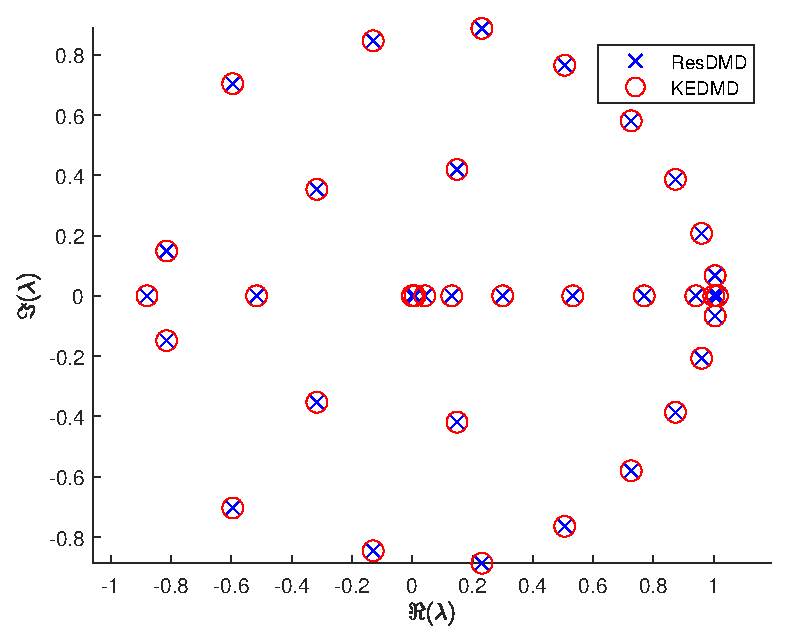
\includegraphics[width=0.55\linewidth]{../code/figures/gauss_map/kernelized/KEDMD_Gauss-Legendre.eps}
\caption{Output of the ResDMD ad K-EDMD algorithm for the Gauss iterated map problem, when using a number of snapshots pairs $M = 40$ equal to the size $K$ of the dictionary, and the kernel defined by the dictionary. The firs $K$ Legendre polynomials are used as a dictionary and the Gauss-Legendre quadrature points as initial snapshots.}
\label{fig_kedmd_vs_edmd}
\end{figure}

Finally, to analyse the effectiveness of the procedure for extracting a dictionary from a general-purpose kernel, we applied the two-stages Kernelized ResDMD algorithm with a RBF kernel. Let us observe that the RBF kernel can be seen as the inner product of an infinite polynomial dictionary, hence we do not have any constraint on the number of snapshot datapoints. As snapshot data for the first stage, we considered $M' = 1000$ Montecarlo quadrature nodes and we extracted the $K' = 40$ dominant eigenpairs using the K-EDMD algorithm. In the second stage, we applied the ResDMD algorithm using the dictionary in output of the K-EDMD algorithm and $M''=1000$ Gauss-Legendre quadrature points as snapshot data. The tolerance employed in K-ResDMD was $\varepsilon = 0.01$. As suggested in \cite{colbrook_rigorous_2021}, we also employed the following common practices:
\begin{itemize}
    \item the constant $\sigma$ of the RBF kernel $\kappa(\vb{x}, \vb{y}) = \exp(-\norm{\vb{x}-\vb{y}}^2 / \sigma^2)$ was set as the average $\ell^2$-norm of the snapshot data after it is shifted to have mean zero.
    \item the gramian matrices of the first stage $\hat{\vb*{G}} = \sqrt{\vb*{W}}\Psi_0\Psi_0^*\sqrt{\vb*{W}}$ and  $\hat{\vb*{A}} = \sqrt{\vb*{W}}\Psi_1\Psi_0^*\sqrt{\vb*{W}}$ are both ill conditioned, with a conditioning number of the order $10^{20}$ and a numerical rank between $40$ and $50$ (their size is $M'=1000$). Therefore, we added regularization in the form $\hat{\vb*{G}} = \hat{\vb*{G}} + \eta \lVert\hat{\vb*{G}}\rVert_F \vb*{I}$ where $\eta = 10^{-16}$. 
\end{itemize}
\Cref{fig_2steps_kedmd} shows the results of the above described procedure. The pseudospectral contour lines computed in \Cref{sect_gauss_iterated_map} are plotted as a reference to evaluate the quality of the approximated eigenvalues. It can be observed that the approximated eigenvalues returned by the K-ResDMD via the two-step extraction procedure are very similar to the ones shown in \Cref{gauss_pseudospectrum_convergence}, obtained using the ResDMD, and they all lie inside the $0.01$-pseudospectrum approximation previously computed. However, the eigenvalues shown in \Cref{fig_2steps_kedmd} did not require a hand-crafted dictionary in input to the algorithm, but employed the general-purpose RBF kernel with the scaling factor $\sigma$ determined using the data. 

\begin{figure}[h]
\centering
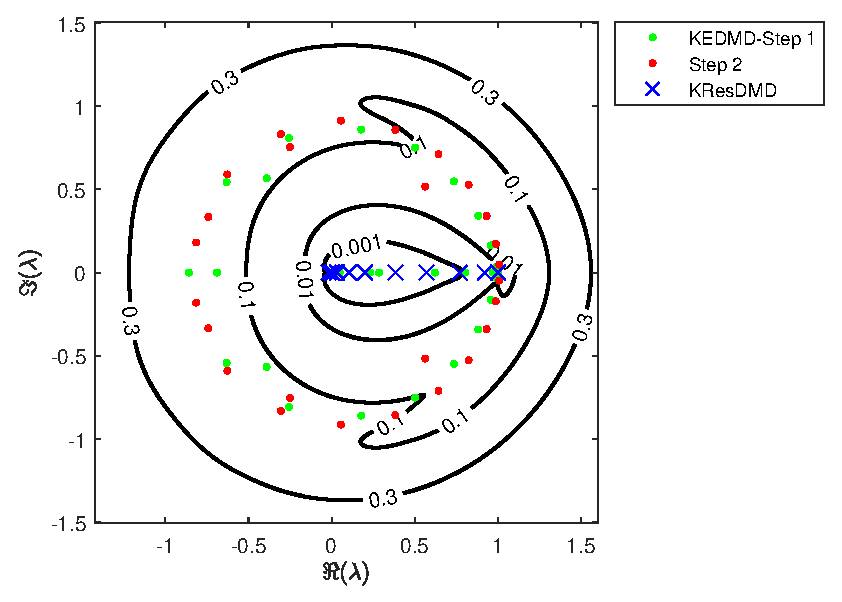
\includegraphics[width=0.70\linewidth]{../code/figures/gauss_map/kernelized/KEDMD_2step_rbf_Montecarlo.eps}
\caption{Eigenvalues approximation for the Gauss iterated map problem, obtained using the two-step procedure described in \Cref{alg_kresdmd}. Green dots show the $K'=40$ dominant eigenvalues computed in the first step. Eigenvalues returned in the second steps are represented as red dots and blue crosses, where blue crosses show the eigenvalues retained by K-ResDMD with tolerance $\epsilon = 0.01$. The pseudospectral contour lines computed in \Cref{sect_gauss_iterated_map} are also plotted as a reference.}
\label{fig_2steps_kedmd}
\end{figure}
